\documentclass{beamer}
\usepackage[utf8]{inputenc}

\usetheme{Madrid}
\usecolortheme{default}
\usepackage{amsmath,amssymb,amsfonts,amsthm}
\usepackage{txfonts}
\usepackage{tkz-euclide}
\usepackage{listings}
\usepackage{adjustbox}
\usepackage{array}
\usepackage{tabularx}
\usepackage{gvv}
\usepackage{lmodern}
\usepackage{circuitikz}
\usepackage{tikz}
\usepackage{graphicx}

\setbeamertemplate{page number in head/foot}[totalframenumber]

\usepackage{tcolorbox}
\tcbuselibrary{minted,breakable,xparse,skins}



\definecolor{bg}{gray}{0.95}
\DeclareTCBListing{mintedbox}{O{}m!O{}}{%
  breakable=true,
  listing engine=minted,
  listing only,
  minted language=#2,
  minted style=default,
  minted options={%
    linenos,
    gobble=0,
    breaklines=true,
    breakafter=,,
    fontsize=\small,
    numbersep=8pt,
    #1},
  boxsep=0pt,
  left skip=0pt,
  right skip=0pt,
  left=25pt,
  right=0pt,
  top=3pt,
  bottom=3pt,
  arc=5pt,
  leftrule=0pt,
  rightrule=0pt,
  bottomrule=2pt,
  toprule=2pt,
  colback=bg,
  colframe=orange!70,
  enhanced,
  overlay={%
    \begin{tcbclipinterior}
    \fill[orange!20!white] (frame.south west) rectangle ([xshift=20pt]frame.north west);
    \end{tcbclipinterior}},
  #3,
}
\lstset{
    language=C,
    basicstyle=\ttfamily\small,
    keywordstyle=\color{blue},
    stringstyle=\color{orange},
    commentstyle=\color{green!60!black},
    numbers=left,
    numberstyle=\tiny\color{gray},
    breaklines=true,
    showstringspaces=false,
}
\begin{document}

\title 
{2.4.29}
\date{August 26,2025}


\author 
{Kavin B-EE25BTECH11033}






\frame{\titlepage}
\begin{frame}{Question}
The points $\vec{A}(2, 9), \vec{B}(a, 5) $ and $\vec{C}(5, 5)$ are the vertices of a triangle $\vec{ABC}$ right angled at $\vec{B}$. Find the values of a and hence the area of $\triangle \vec{ABC}$.
\end{frame}



\begin{frame}{Theoretical Solution}

Given the points,
\begin{align}
    \vec{A}=\begin{myvec}{2\\9}\end{myvec}\ \ 
    \vec{B}=\begin{myvec}{a\\5}\end{myvec}\ \ 
    \vec{C}=\begin{myvec}{5\\5}\end{myvec}
\end{align}
Also it is given that the triangle $\vec{ABC}$ right angled at $\vec{B}$.\\
\\
$\therefore$ The vectors $(\vec{A}-\vec{B})$ and $(\vec{C}-\vec{B})$ are perpendicular.\\
\end{frame}

\begin{frame}{Formulae}
\textbf{The angle $\theta$ between vectors $(\vec{A}-\vec{B}), (\vec{C}-\vec{B})$, is given by } 
\begin{align}
	\label{eq:angle-inner}
		\cos\theta=\frac{{(\vec{A}-\vec{B})^{\top}}{(\vec{C}-\vec{B})}}{\norm{\vec{A}-\vec{B}}\norm{\vec{C}-\vec{B}}}
\end{align}
\end{frame}


\begin{frame}{Theoretical Solution}
Here $\theta$ = $90\degree$.

\begin{align}
\implies {(\vec{A}-\vec{B})^{\top}}{(\vec{C}-\vec{B})} = 0
\end{align}\\
\begin{center}
$\vec{A}$ - $\vec{B}$ = $\myvec{2-a\\4}$
\end{center}
\begin{center}
$\vec{C}$ - $\vec{B}$ = $\myvec{5-a\\0}$
\end{center}

\end{frame}

\begin{frame}{Theoretical Solution}

\begin{align}
    \implies\myvec{2-a\\4}^{\top}\myvec{5-a\\0} = 0\\
    \implies\myvec{2-a & 4}\myvec{5-a\\0} = 0\\
    \implies \brak{2-a}\brak{5-a} + \brak{4\times0} = 0\\
    \implies \brak{2-a}\brak{5-a} = 0
\end{align}
\begin{align}
    \implies a = 2
\end{align}
\\
Here $a = 5$ is not considered because when $a = 5$, the points $\vec{B}$ and $\vec{C}$ will be the same and hence a triangle cannot be formed.\\
\begin{center}
$\vec{B}=\begin{myvec}{2\\5}\end{myvec}$
\end{center}

\end{frame}
\begin{frame}{Formulae}
\textbf{The area of $\triangle ABC$ is given by}
		\begin{align}
			Area = \frac{1}{2}\norm{{\brak{\vec{A}-\vec{B}}\times \brak{\vec{A}-\vec{C}}}}
		\end{align}
\end{frame}

\begin{frame}{Theoretical Solution}
\begin{center}
    \brak{\vec{A}-\vec{B}} =$\myvec{0\\4}$\\
    \brak{\vec{A}-\vec{C}} = $\myvec{-3\\4}$
\end{center}
\\
\begin{align}
\implies Area = \frac{1}{2}\norm{\myvec{0\\4}\times \myvec{-3\\4}}
\end{align}
\begin{align}
\implies Area = \frac{1}{2}\norm{0 + 12}
\end{align}
\begin{align}
\implies Area = 6
\end{align}\\
Hence the area of $\triangle \vec{ABC}$ is $6$ sq.units.\\

\end{frame}


\begin{frame}[fragile]
    \frametitle{C Code - A function to find the value of a}

    \begin{lstlisting}

#include <stdio.h>
#include <math.h>
#include <stdlib.h>

typedef struct {
    double x;
    double y;
} Point;

typedef struct {
    int count;
    double solution1;
    double solution2;
} Solutions;

    \end{lstlisting}
\end{frame}

\begin{frame}[fragile]
    \frametitle{C Code - A function to find the value of a}

    \begin{lstlisting}
Solutions solveForA(Point A, double B_y, Point C) {
    Solutions result = {0, 0.0, 0.0};
    
    double P = 1.0;
    double Q = -(A.x + C.x);
    double R = (A.x * C.x) + (A.y - B_y) * (C.y - B_y);
    double discriminant = Q*Q - 4*P*R;

    if (discriminant < 0) {
        return result;
    }

    double a1 = (-Q + sqrt(discriminant)) / (2*P);
    double a2 = (-Q - sqrt(discriminant)) / (2*P);

    \end{lstlisting}
\end{frame}

\begin{frame}[fragile]
    \frametitle{C Code - A function to find the value of a}

    \begin{lstlisting}
    int a1_is_valid = !(a1 == A.x && B_y == A.y) && !(a1 == C.x && B_y == C.y);
    int a2_is_valid = !(a2 == A.x && B_y == A.y) && !(a2 == C.x && B_y == C.y);
    if (a1_is_valid) {
        result.solution1 = a1;
        result.count++;
    }   
    if (discriminant > 1e-9 && a2_is_valid) {
        if (result.count == 0) {
            result.solution1 = a2;
        } else {
            result.solution2 = a2;
        }
        result.count++;
    }
    return result;
}

    \end{lstlisting}
\end{frame}

\begin{frame}[fragile]
    \frametitle{C Code - A function to find the value of a}

    \begin{lstlisting}

double getValidA() {
    Point A = {2.0, 9.0};
    Point C = {5.0, 5.0};
    double B_y = 5.0;
    
    Solutions solutions = solveForA(A, B_y, C);
    
    if (solutions.count > 0) {
        return solutions.solution1;
    }
    
    return 2.0;
}

    \end{lstlisting}
\end{frame}


\begin{frame}[fragile]
    \frametitle{Python Code}
    \begin{lstlisting}
import numpy as np
import numpy.linalg as LA
import matplotlib.pyplot as plt
import ctypes
import os

# Load the shared library
lib = ctypes.CDLL('./code.so')

# Define C types matching the exact structure
class Point(ctypes.Structure):
    _fields_ = [("x", ctypes.c_double),
                ("y", ctypes.c_double)]

class Solutions(ctypes.Structure):
    _fields_ = [("count", ctypes.c_int),
                ("solution1", ctypes.c_double),
                ("solution2", ctypes.c_double)]

    \end{lstlisting}
\end{frame}

\begin{frame}[fragile]
    \frametitle{Python Code}
    \begin{lstlisting}
# Set up function prototypes exactly as in C
lib.solveForA.argtypes = [Point, ctypes.c_double, Point]
lib.solveForA.restype = Solutions

lib.getValidA.argtypes = []
lib.getValidA.restype = ctypes.c_double

# Get the value of a from C library using the exact function
a_value = lib.getValidA()
print(f"Value of a from C library: {a_value}")
# Define points
A = np.array([2, 9])
B = np.array([a_value, 5])
C = np.array([5, 5])
print(f"Coordinates:")
print(f"A({A[0]}, {A[1]})")
print(f"B({B[0]}, {B[1]})")
print(f"C({C[0]}, {C[1]})")

    \end{lstlisting}
\end{frame}

\begin{frame}[fragile]
    \frametitle{Python Code}
    \begin{lstlisting}
# Function to generate line points
def line_gen(P, Q):
    return np.column_stack((P, Q))

# Calculate triangle properties
c = LA.norm(A - B)
a = LA.norm(B - C)
b = LA.norm(C - A)
print(f"\nSide lengths:")
print(f"AB = {c:.2f}")
print(f"BC = {a:.2f}")
print(f"CA = {b:.2f}")



    \end{lstlisting}
\end{frame}

\begin{frame}[fragile]
    \frametitle{Python Code}
    \begin{lstlisting}
# Calculate area (since it's right-angled at B)
area = 0.5 * a * c
print(f"\nArea of triangle ABC: {area:.2f}")

# Generate lines
x_AB = line_gen(A, B)
x_BC = line_gen(B, C)
x_CA = line_gen(C, A)

# Plotting
plt.figure(figsize=(10, 8))
plt.plot(x_AB[0,:], x_AB[1,:], label='$AB$', linewidth=3, color='blue')
plt.plot(x_BC[0,:], x_BC[1,:], label='$BC$', linewidth=3, color='green')
plt.plot(x_CA[0,:], x_CA[1,:], label='$CA$', linewidth=3, color='red')

    \end{lstlisting}
\end{frame}
\begin{frame}[fragile]
    \frametitle{Python Code}
    \begin{lstlisting}
# Labeling the coordinates
tri_coords = np.column_stack((A, B, C))
plt.scatter(tri_coords[0,:], tri_coords[1,:], color='black', s=150, zorder=5)

vert_labels = ['A','B','C']
for i, txt in enumerate(vert_labels):
    plt.annotate(txt, 
                 (tri_coords[0,i], tri_coords[1,i]),
                 textcoords="offset points",
                 xytext=(0,15),
                 ha='center',
                 fontsize=14,
                 fontweight='bold',
                 bbox=dict(boxstyle="round,pad=0.3", facecolor="yellow", alpha=0.7))

    \end{lstlisting}
\end{frame}
\begin{frame}[fragile]
    \frametitle{Python Code}
    \begin{lstlisting}
plt.xlabel('$x$', fontsize=14)
plt.ylabel('$y$', fontsize=14)
plt.legend(loc='upper right', fontsize=12)
plt.grid(True, alpha=0.3, linestyle='--')
plt.axis('equal')

# Set appropriate limits with some padding
plt.xlim(min(tri_coords[0,:]) - 1, max(tri_coords[0,:]) + 1)
plt.ylim(min(tri_coords[1,:]) - 1, max(tri_coords[1,:]) + 1)
    \end{lstlisting}
\end{frame}

\begin{frame}[fragile]
    \frametitle{Python Code}
    \begin{lstlisting}
# Add right angle marker at B
angle_x = B[0] + 0.5
angle_y = B[1] + 0.5
plt.plot([B[0], angle_x], [B[1], B[1]], 'k--', alpha=0.5)
plt.plot([B[0], B[0]], [B[1], angle_y], 'k--', alpha=0.5)
plt.text(B[0] + 0.3, B[1] + 0.3, '90°', fontsize=12, fontweight='bold')

plt.tight_layout()
plt.savefig('../figs/fig.png')
plt.show()

    \end{lstlisting}
\end{frame}

\begin{frame}{Plot}
    \centering
    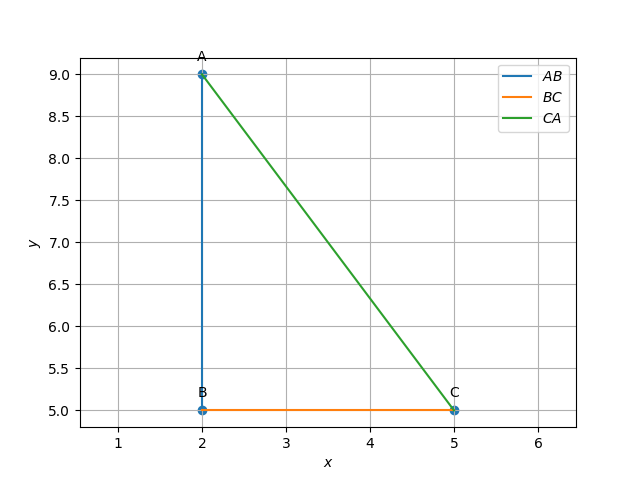
\includegraphics[width=\columnwidth, height=0.8\textheight, keepaspectratio]{figs/fig.png}     
\end{frame}


\end{document}